\chapter{Part B: Yield Curve}
Developer: Yann Renoux

\noindent Validator: Joseph Perez


%DEVELOPER WRITES THIS PART --->

\section{Requirements}


\par All the formulas used in this project are based on risk-neutral valuation
and non-arbitrage, with a risk free rate. Hence whatever the product we consider,
we need to have a solid base class to handle the needs of classes that define products.
This object has to gather market data in the form of a market yield curve and provide the basic methods expected.
Such methods go from getting the spot zero coupon -- \emph{ZC} -- rate for a certain
maturity, the discount factor to present value future cash-flows or forward rates to evaluate
such future flows. But these methods can also include different interest composition, such as annual or continuous.

\subsection{Other methods we added for risk management purposes}

\par In addition to the basic methods required, we have added a shift and a rotation to model the 2 first
known factors of the Principal Component analysis on the term structure of a yield curve:

\begin{figure}
\begin{center}
        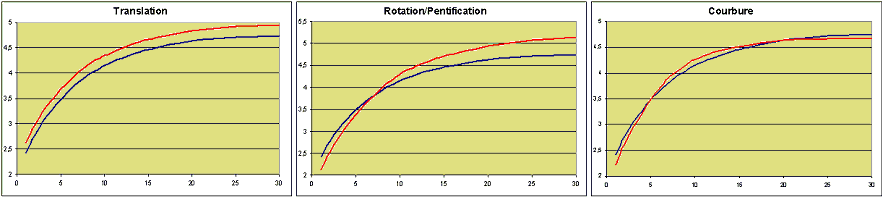
\includegraphics[width=12cm]{3mvts.png}
        \caption{3 first axis of the PCA (95\% of the variance): Shift, Rotation and Curvature}
\end{center}
\end{figure}


\par This will be very useful in term of risk management, as we know that all the rates bear a correlation and
the term structure is very unlikely to revert from one day to the other.

\par For instance, a yield curve is a set of data points with ascending maturities, related to some fixed-income product that provides a yield.
In practice, the short end of the curve comes from the ZCB's, and the rest is from the swap market. As those 2 evolve in a different space, the object needs to rotate the space of swaps into ZC rates.

\par We mentioned the methods we want the yield curve to be able to perform, but not what it will use as base data.
We have decided to store the term structure from the market curve, which is made
of zero coupon rates for short maturities -- 0.25, 0.5 and 1 year for the US market --
and swap rates -- from 2 to 10, 15, 20 and 30 years in the same market. As these rates do not come from the same
sort of product, they do not belong in the same space, hence a transformation needs to be done to have them in
comparable values: the class must be able to do the rotation transparently.

\subsection{From swap rates to ZC rates}
\par Consider a swap with notional $N$ such that:
\begin{itemize}
\item the floating leg delivers $m$ flows at dates $T_{j}$ for $j=1...m$
\item the fix leg with rate $C$ delivers $n$ flows at dates
$T_{ki}$ for $i=1...n$, $k$ being the ratio between the annual frequency of payment of the floating versus the fix leg, so that $kn=m$.
\end{itemize}

\par The so-called zero-coupons method provides a way to evaluate this vanilla swap, being equal to that of:
\begin{itemize}
\item a fixed coupon bond with same maturity and notional
\item minus the swap notional (a swap does not exchange principal).
\end{itemize}


\par Hence, defining $B(t,T_{ki}) $ the value at $t$ of a ZC paying 1 dollar at $T_{ki}$, we can write:
$$ SWAP_{t}=N \left(\sum_{i=1}^{n}C B(t, T_{ki})+B(t, T_{m}) \right)-N $$
where at any given date, the fix rate $C$ is the par swap rate, giving the NPV equal to zero.

\par Thus at $t$, each swap rate $s(t,.)$ verifies:
$$1=\sum_{i=1}^{m-1} \frac{s(t,m)}{\left(1+R(t,i)\right)^i} + \frac{1+s(t,m)}{\left(1+R(t,m)\right)^m}$$
Writing them up for all known maturities between 1 and $m$, we get matricially:

$$\left(
\begin{array}{ccccc}
1+s(t,1) & 0 & 0 &  & 0 \\
s(t, 2) & 1+s(t,2) & 0 & \ddots & \vdots \\
\vdots & \ddots & \ddots & & 0 \\
s(t,m-1) & & s(t,m-1)& 1+s(t,m-1)& 0 \\
s(t,m) & \cdots & \cdots & s(t,m) & 1+s(t,m) \\
\end{array}
\right) \left(
\begin{array}{c}
\frac{1}{\left(1+R(t,1)\right)^1} \\
\\
\vdots\\
\\
\frac{1}{\left(1+R(t,m)\right)^m} \\
\end{array}
\right)= \left(
\begin{array}{c}
1 \\
\\
\vdots\\
\\
1 \\
\end{array}
\right)
$$
that is to say:
$$ A(t) \left(
\begin{array}{c}
\frac{1}{\left(1+R(t,m)\right)^1} \\
\\
\vdots\\
\\
\frac{1}{\left(1+R(t,m)\right)^m} \\
\end{array}
\right)= \left(
\begin{array}{c}
1 \\
\\
\vdots\\
\\
1 \\
\end{array}
\right)
$$hence
$$\left(
\begin{array}{c}
\frac{1}{\left(1+R(t,1)\right)^1} \\
\\
\vdots\\
\\
\frac{1}{\left(1+R(t,m)\right)^m} \\
\end{array}
\right)= A(t)^{-1} \left(
\begin{array}{c}
1 \\
\\
\vdots\\
\\
1 \\
\end{array}
\right)
$$

\par Hence if we have all the intermediary points, we can just back out the ZC rates while solving an easy triangular system.
We will come back to the assumptions we made here later.


\section{Design }


\subsection{Approach}
%<high-level description of the design>
\par Prior to studying what a yield curve is, a simplier object should be defined, the yield point. Its 4 members are :
\begin{itemize}
    \item a type (Cash or Swap - but can be extended to other instruments),
    \item a rate,
    \item a maturity in years, and
    \item a Daycount convention (defaulted to Actual/360, the most common convention for USD Libor swap rates).
\end{itemize}
\par Note that the maturity is not a date, as commonly people talk about the 5 years swap rate or the 1 year ZC rate. The yield curve will be able to transform one into the other so that the user can use both.

\par A yield curve is then a valarray of yield points, but can be assigned a flat rate in anotehr constructor. At the construction, we need to make sure that the transformation is being made according to the method exposed earlier, so that the user can build a yield curve with several types of rates and be able to back out the tools without adding any line of code. In addition to that, the yield curve object also has a name field, so that the user can define a "USD Libor Curve" or a "EUR Libor Curve".

\subsection{Choices}
%<any important design choices you made, e.g. data structures, class hierarchy, algorithm, etc. and a justification for the decision>
\par As we said earlier, to get the ZC rates from the swap rates, we need to solve a triangular system. The 1 year swap rate is the 1 year zero coupon rate (write the formula...), but then it depends on what is the type of swap rate we are talking about. Say we have market quotes on semi annual swap rates, then we would need the 1.5 year swap rate to back out the 1.5 year ZC rate as we know the 1 year one. Here the choice was made to consider annual swap rates -- as in the Bloomberg quotes file provided, as well as a linear interpolation when needed. For instance, we have here solved the 1-10 years issue as all maturities there follow each other, but what for the rest ? Well the 12 years swap rate is taken as the weighted average of the nearest higher and lower rate known, here 15 and 10 years. We did not code splines interpolation method, as we thought that was not the main emergency in the class. As a result, we face a little bump on the reconstruction after the 10 year ZC rate due to this approximation:

\begin{figure}
\begin{center}
        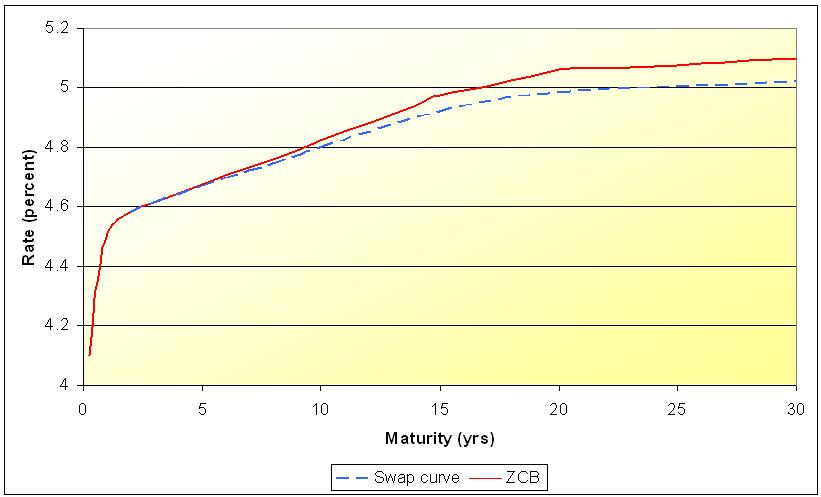
\includegraphics[width=12cm]{yc.jpg}
        \caption{ZC curve reconstruction from annual swap rates from 1-10 years, 15, 20 and 30 years.}
\end{center}
\end{figure}


\par We supposed that the user provides rates non ordered by maturity or type, then it does the sorting by itself. All the same if the user does not enter all rates, the swap to ZC private method does all what is needed to handle it.



\subsection{Methods}

\par On top of the necessay methods already mentionned (discount factor, forward rate, sorting, inverting swap to ZC, shift or rotate the curve, etc.), the yield curve has an output operator "$<<$" for easy checking, as well as a comparison one "==".

\subsection{Unit tests}

%<short descriptions of each subtest>
\par We used the file we provided from BBG (US Yield Curve "IYC", October, 5th, 2005). We computed zero coupons and output them as we saw earlier, computed some spot rates, discount factors, forward rates for different maturities in years or date, and changed the conventions. We have compared them to the calculus by hand in Excel, to make sure the results were coherent, as this class needs to be accurate for all the forthcoming ones.

\begin{figure}[htbp]
\begin{center}
        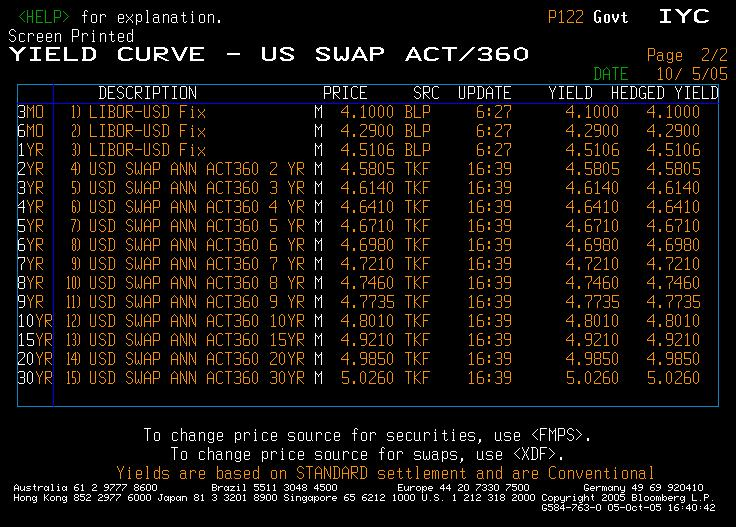
\includegraphics[width=10cm]{YC_RATES.jpg}
        \caption{Bloomberg YC Data for USA}
\end{center}
\end{figure}


\begin{figure}[htbp]
\begin{center}
        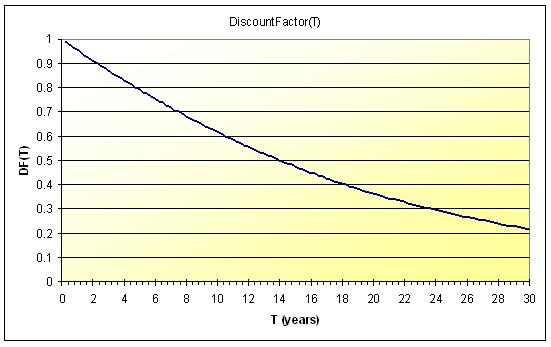
\includegraphics[width=12cm]{DF.jpg}
        \caption{Graph of the continuously compounded discount factors up to 30 years}
\end{center}
\end{figure}

\par We can note that the decreasing effect of the discount factor seems to be appropriate. See section 4. of the module to visualize the tests ran, as well as the validation part.

\begin{figure}[htbp]
\begin{center}
        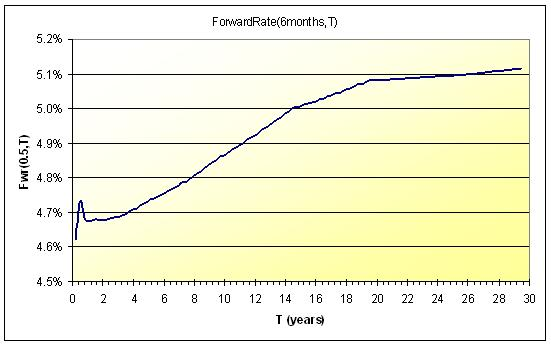
\includegraphics[width=12cm]{fwdRates.jpg}
        \caption{Graph of the forward rates starting in 6 months}
\end{center}
\end{figure}


\par On the forward rate graph, there is a break at (6m,6m) which corresponds to the change from ZC to swap rates, indeed the interpolation method has a huge impact on the forward rates. See \textit{http://www.riskworx.com/insights/interpolation/interpolation.htm} for more explanation. We conclude that for our purpose, the forward curve is satisfactory, and as mentionned, could be improved by improving the interpolation method.

\par To finish, we tested the several methods, spot, discount factor, forward rate and compared to the calculus we should have, just by using the yield curve and calculating the expected prices. They were all in line -- see the mainyieldcurve program in the test directory for more details. Results in in data/rates.xls

\subsection{Performance}

\par We have mentionned various assumptions, and their addition would increase the computation time. For instance, the flexibility of swaps frequency, or the splines interpolation.

\par But as is, aside of the valarray that might not be "the" efficient structure for a too small amount of data, some methods or storage could be improved. As an example, all the getSwapRates - maybe we could store them separately at the construction and avoid needing to find them, etc.
Also, the getSequentSwapRates, used to the first part of the curve 1Y-10Y, is used only to be able to know whether or not to interpolate. It might be redundant if the list of swaps we get for the matrix invertion was better seen.


%VALIDATOR WRITES THIS PART --->

\section{Validation}


\subsection{Approach}
A way to validate the construction of a yield curve was to compute prices of zero coupon bond of short maturity and the swap rates with a yieldCurve object and compare them to the input we gave to construct it. They matched.
The other validation method was to use the yield curve in every other section. As with the other objects (bond, montecarlo...) we got good results it means that the yield curve was well defined.
%\subsection{Pitfalls}

%<i.e. what bugs were found>
